\documentclass[tikz,border=10pt]{standalone}
\usepackage{amsmath}
\usetikzlibrary{calc}

\begin{document}
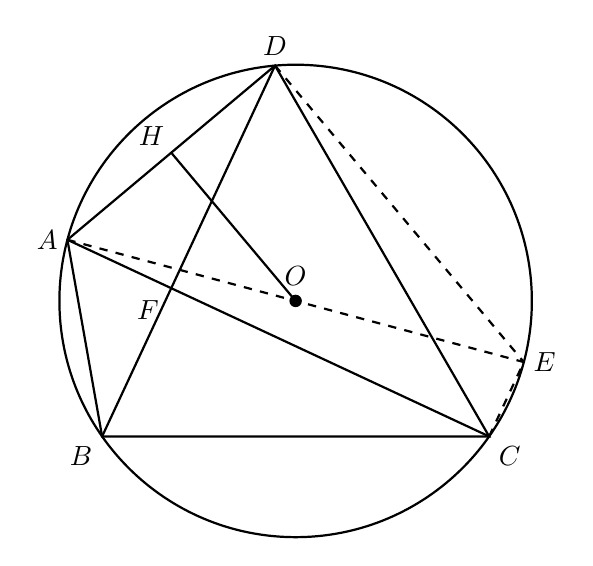
\begin{tikzpicture}[>=stealth, scale=1.5]
    % 严格计算点位：保证 AC 垂直 BD，且 E 和 C 保持恰当的可见间距
    \coordinate (O) at (0,0);
    \coordinate (A) at (165:2);
    \coordinate (E) at (-15:2); % AE 为直径
    \coordinate (C) at (-35:2); % 在 E 下方稍稍远离 (间距 20 度)
    \coordinate (D) at (95:2);
    \coordinate (B) at (215:2); % 此时 A+C 的角度和为 130，B+D 为 310，差值为 180，保证绝对垂直
    
    % H为AD中点
    \coordinate (H) at (130:{2*cos(35)});
    \coordinate (F) at (intersection of A--C and B--D);

    % 绘制外接圆
    \draw[thick] (O) circle (2);

    % 绘制实线段
    \draw[thick] (A) -- (B) -- (C) -- (D) -- cycle;
    \draw[thick] (A) -- (C);
    \draw[thick] (B) -- (D);
    \draw[thick] (O) -- (H);

    % 绘制虚线辅助线
    \draw[dashed, thick] (A) -- (E);
    \draw[dashed, thick] (D) -- (E);
    \draw[dashed, thick] (C) -- (E);

    % 标注字母
    \fill (O) circle (1.5pt) node[above=2pt] {$O$};
    \node[left] at (A) {$A$};
    \node[below left] at (B) {$B$};
    \node[below right] at (C) {$C$};
    \node[above] at (D) {$D$};
    \node[right] at (E) {$E$};
    \node[above left=-1pt] at (H) {$H$};
    \node[below left=1pt] at (F) {$F$};

\end{tikzpicture}
\end{document}